Modultesten er udarbejdet ved at lave et testprogram. Testprogrammet ses i source filen og sætter en test pin høj, figur \ref{lab:test_maaling} viser en test måling og det kan konkluderes at PSoC programmet fungerer efter hensigten, da billedet viser at programmet går korrekt ind i ISR rutinen.    


\subsubsection*{Source fil}
\begin{lstlisting}[language=C]
CY_ISR(P_PIR)
{
    TEST_Write(1);
    TEST_Write(0); 
}
\end{lstlisting}


\begin{figure}[H]
\centering
{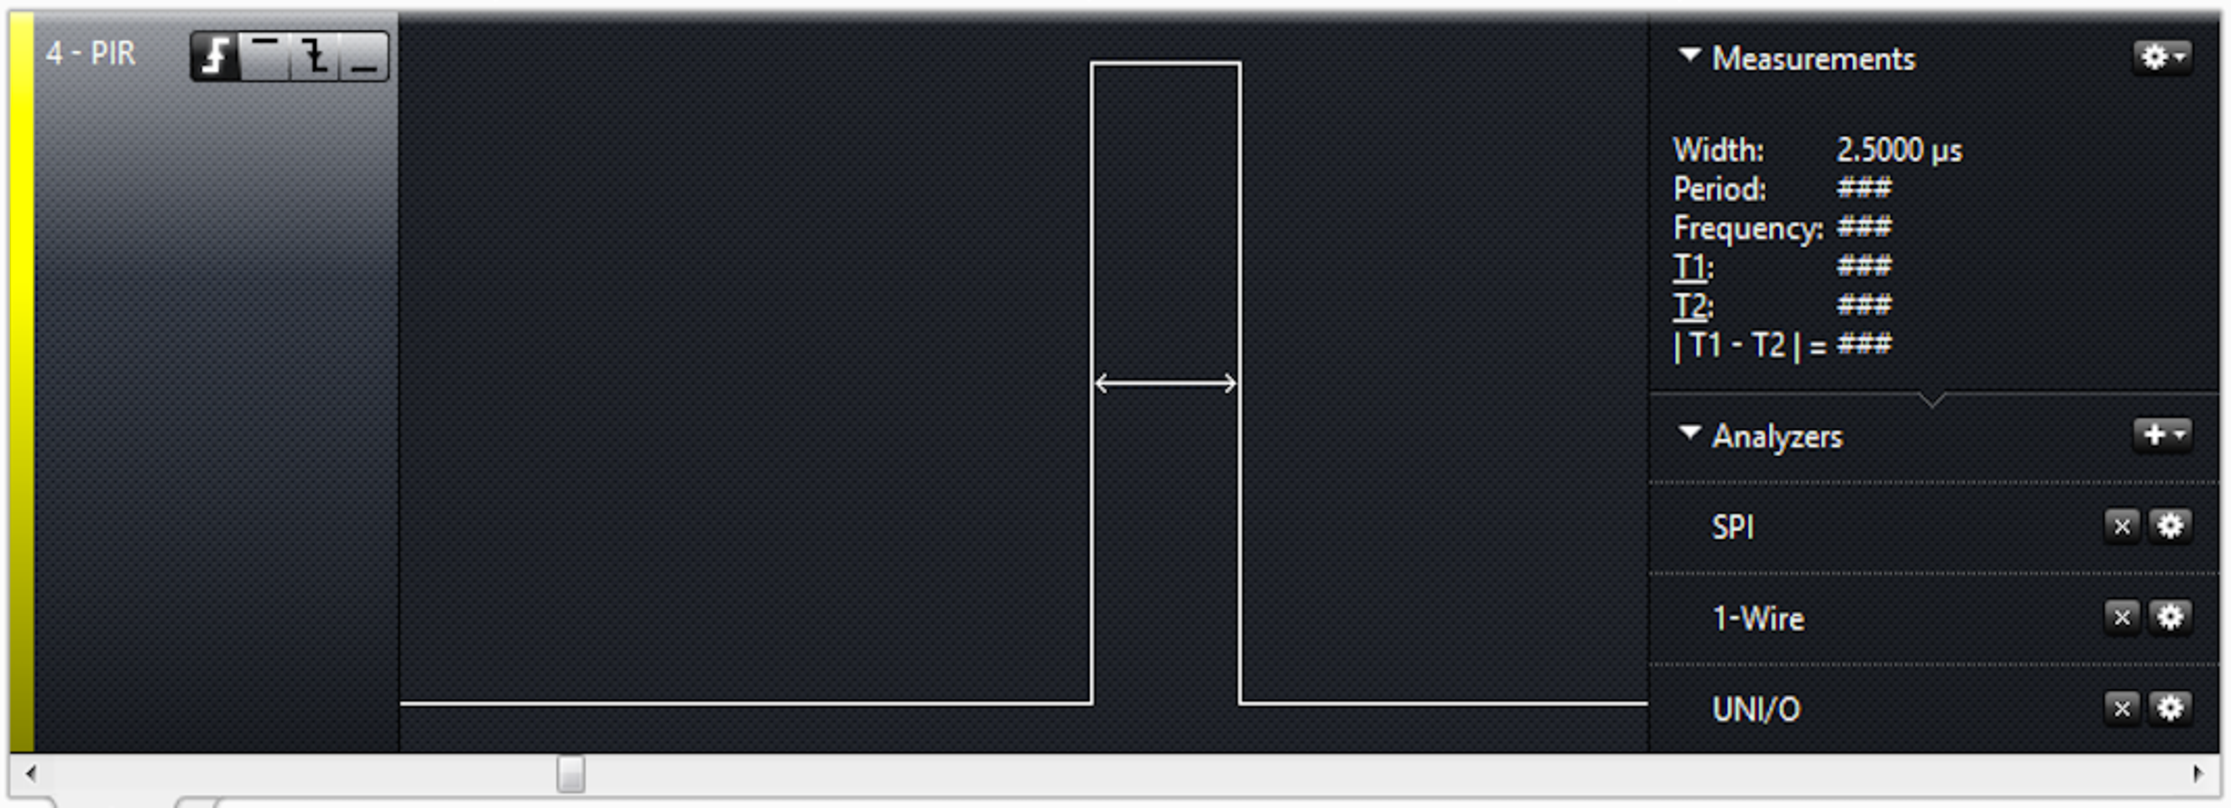
\includegraphics[width=0.60\textwidth]{filer/modultest/billeder/pir_testmaaling}}
\caption{Analyse billedet for pir aktivering}
\label{lab:test_maaling}
\end{figure}

